% =====================================================================
% PagedAttention in MiniTorch  --  Project Poster
% Size: 36" wide x 42" tall (portrait)
% Build: latexmk -pdf poster.tex   (or)   pdflatex poster.tex
% =====================================================================
\documentclass[17pt]{extarticle}

\usepackage[paperwidth=36in, paperheight=42in,
                                    left=0.45in, right=0.45in, top=0.35in, bottom=0.35in]{geometry}

\usepackage{graphicx}
\usepackage{amsmath, amssymb}
\usepackage{booktabs}
\usepackage{array}
\usepackage[table]{xcolor}
\usepackage[most]{tcolorbox}
\usepackage{enumitem}
\usepackage{fontawesome5}
\usepackage{helvet}
\usepackage{tikz}

\renewcommand{\familydefault}{\sfdefault}
\pagestyle{empty}
\setlength{\parindent}{0pt}
\setlength{\parskip}{0pt}

% ---------------------------------------------------------------------
% Colors
% ---------------------------------------------------------------------
\definecolor{navyDeep}{HTML}{0C2340}
\definecolor{signalBlue}{HTML}{1E5FA8}
\definecolor{signalTeal}{HTML}{17817A}
\definecolor{signalGold}{HTML}{A96D00}
\definecolor{signalRed}{HTML}{C45757}
\definecolor{signalSlate}{HTML}{5E7087}
\definecolor{paperBg}{HTML}{F3F6FA}
\definecolor{panelBg}{HTML}{EEF3F8}
\definecolor{softBorder}{HTML}{CCD5E0}
\definecolor{inkDark}{HTML}{243242}

\pagecolor{paperBg}
\color{inkDark}

\setlist[itemize]{leftmargin=*, itemsep=11pt, topsep=8pt}
\setlist[enumerate]{leftmargin=*, itemsep=11pt, topsep=8pt}

\newlength{\PosterColumnHeight}
\setlength{\PosterColumnHeight}{35.45in}

% ---------------------------------------------------------------------
% Shared box styles
% ---------------------------------------------------------------------
\newtcolorbox{posterbox}[3][]{%
      enhanced,
      breakable=false,
      colback=white,
      colframe=#2!40!softBorder,
      boxrule=0.9pt,
      arc=4mm,
      left=3.2mm, right=3.2mm, top=4.8mm, bottom=3.2mm,
      title={\strut\textbf{#3}},
      fonttitle=\LARGE\bfseries,
      coltitle=white,
      colbacktitle=#2,
      attach boxed title to top left={xshift=7mm, yshift*=-3mm},
      boxed title style={arc=3mm, boxrule=0pt, colback=#2,
                                                             left=4mm, right=4mm, top=2mm, bottom=2mm},
      borderline west={5pt}{0pt}{#2},
      before skip=0pt,
      after skip=0pt,
      drop fuzzy shadow=black!8,
      #1
}

\newtcolorbox{metricbox}[1]{%
      enhanced,
      colback=white,
      colframe=#1!40!softBorder,
      boxrule=0.9pt,
      arc=4mm,
      left=3.6mm, right=3.6mm, top=3.2mm, bottom=3.2mm,
      borderline west={5pt}{0pt}{#1},
      drop fuzzy shadow=black!8,
      before skip=0pt,
      after skip=0pt
}

\newcommand{\pill}[2]{%
      \tcbox[on line, boxrule=0pt, arc=3mm,
            colback=#1!85!black, colframe=#1!85!black,
            left=3mm, right=3mm, top=1.2mm, bottom=1.2mm]{%
            \color{white}\small\bfseries #2}%
}

\newcommand{\metriccard}[4]{%
\begin{metricbox}{#1}
\centering
{\fontsize{40.5}{42.5}\selectfont\bfseries\textcolor{#1}{#2}}\\[2pt]
{\Large\bfseries #3}\\[2pt]
{\large\color{signalSlate} #4}
\end{metricbox}}

\newcommand{\figpanel}[2][3.85in]{%
\begin{tcolorbox}[enhanced, boxrule=0.6pt, arc=3mm,
      colback=panelBg, colframe=softBorder,
      left=1.5mm, right=1.5mm, top=1.5mm, bottom=1.5mm,
      before skip=0pt, after skip=0pt]
\centering
\includegraphics[width=0.985\linewidth, height=#1, keepaspectratio]{#2}
\end{tcolorbox}}

\newcommand{\figcaptiontext}[1]{\par\vspace{6pt}{\fontsize{28.2}{33}\selectfont #1}}
\newcommand{\bodycopy}{\fontsize{31.5}{36.8}\selectfont}
\newcommand{\subhead}[1]{\par\vspace{2mm}{\fontsize{30}{35}\selectfont\bfseries\textcolor{navyDeep}{#1}}\par\vspace{1mm}}
\newcommand{\blockgap}{\par\vspace{1.2mm plus 0.55fill}}
\newcommand{\metricstobodygap}{\par\vspace{0.45in}}
\newenvironment{postercolumn}{%
\begin{minipage}[t][\PosterColumnHeight][s]{0.321\linewidth}
\vspace{0pt}%
}{%
\end{minipage}%
}

% ---------------------------------------------------------------------
% Header banner
% ---------------------------------------------------------------------
\newcommand{\HeaderBanner}{%
\begin{tcolorbox}[enhanced, arc=6mm,
      colback=navyDeep, colframe=navyDeep, boxrule=0pt,
      left=15mm, right=15mm, top=6.8mm, bottom=6.8mm,
      before skip=0pt, after skip=3.5mm,
      overlay={
            \fill[signalTeal!85!white, opacity=0.18]
                  ([xshift=-10.5cm]frame.north east) --
                  (frame.north east) --
                  (frame.south east) --
                  ([xshift=-6.5cm]frame.south east) -- cycle;
            \fill[signalGold, opacity=0.18]
                  ([xshift=-3.6cm,yshift=-1.0cm]frame.north east) circle (1.7cm);
            \fill[white, opacity=0.05]
                  ([xshift=-8.2cm,yshift=-0.8cm]frame.north east) circle (1.1cm);
      }]
\color{white}
\begin{minipage}[t]{0.69\linewidth}
{\fontsize{68}{76}\selectfont\bfseries PagedAttention in MiniTorch}\\[3pt]
{\fontsize{28}{34}\selectfont Rigorous Memory, Capacity, Prefix-Reuse, and Branching Results for Block-Granular KV Storage}\\[7pt]
{\fontsize{22}{28}\selectfont \textbf{NingRui Yang} \quad \textbf{Yixiang Dai}}\\[5pt]
{\fontsize{18}{22}\selectfont Carnegie Mellon University \;|\; Electrical \& Computer Engineering \;|\; 11-868 Large Language Model Systems}
\end{minipage}\hfill
\begin{minipage}[t]{0.27\linewidth}\raggedleft
\vspace{1mm}
\pill{signalBlue}{CUDA Kernel}\hspace{2mm}
\pill{signalTeal}{Prefix Cache}\\[3mm]
\pill{signalGold}{Capacity Curves}\hspace{2mm}
\pill{signalRed}{Branch Sharing}\\[7mm]
{\fontsize{18}{23}\selectfont\bfseries The updated codebase evaluates realistic reservation waste, empirical capacity, prefix reuse, and branching-memory savings.}
\end{minipage}
\end{tcolorbox}}

\begin{document}

\HeaderBanner

% =====================================================================
% Metric cards
% =====================================================================
\begin{minipage}[t]{0.192\linewidth}
\vspace{0pt}
\metriccard{signalGold}{96.6\%}{KV Efficiency}{reserved vs. live KV on realistic mix}
\end{minipage}\hfill
\begin{minipage}[t]{0.192\linewidth}
\vspace{0pt}
\metriccard{signalTeal}{2.00x}{Capacity Gain}{vs. \texttt{seq\_len+32} static cap}
\end{minipage}\hfill
\begin{minipage}[t]{0.192\linewidth}
\vspace{0pt}
\metriccard{signalBlue}{1.90x}{Prefix Prefill Speedup}{at 75\% shared prompt}
\end{minipage}\hfill
\begin{minipage}[t]{0.192\linewidth}
\vspace{0pt}
\metriccard{signalRed}{78\%}{Parallel KV Savings}{shared fork vs. naive clone}
\end{minipage}\hfill
\begin{minipage}[t]{0.192\linewidth}
\vspace{0pt}
\metriccard{signalSlate}{79\%}{Beam KV Savings}{winner-takes-all trunk sharing}
\end{minipage}

\metricstobodygap

% =====================================================================
% Three-column poster body
% =====================================================================
\begin{postercolumn}
\begin{posterbox}{navyDeep}{\faLightbulb\ Why This Matters}
\bodycopy
\textbf{KV reservation, not attention math, dominates serving efficiency.} Static allocation pays for a worst-case cap per request:

\begin{tcolorbox}[enhanced, arc=3mm, boxrule=0pt,
      colback=panelBg, left=4mm, right=4mm, top=2.5mm, bottom=2.5mm,
      before skip=4mm, after skip=4mm]
\[
\text{KV}_{\text{static}} = 2 \cdot L \cdot H \cdot d_h \cdot N_{\text{cap}} \cdot B
\]
\end{tcolorbox}

\begin{itemize}
      \item Reserved bytes that never get used directly cap concurrency.
      \item Static waste grows when prompt lengths are non-aligned with the chosen block or cap size.
      \item PagedAttention replaces slabs with reusable blocks and copy-on-write only where branches diverge.
\end{itemize}
\end{posterbox}

\blockgap

\begin{posterbox}{signalBlue}{\faBullseye\ Problem Statement}
\bodycopy
LLM serving is bottlenecked not by attention math but by \textbf{KV-cache memory}. Static contiguous allocation reserves a worst-case slab per request, so most KV bytes are reserved but never used.

\subhead{Goals}
\begin{itemize}
      \item Quantify reserved-vs-used KV waste under a realistic non-aligned workload.
      \item Measure capacity gain, prefix-prefill speedup, and branching-memory savings of paged allocation in MiniTorch + CUDA.
      \item Separate allocator-focused synthetic measurements from claims about end-to-end serving latency.
\end{itemize}
\end{posterbox}

\blockgap

\begin{posterbox}{signalTeal}{\faCogs\ Methodology: What We Built}
\bodycopy
MiniTorch implementation, CUDA decode kernel, and a benchmark harness isolate where paged KV helps.

\subhead{Allocator + sharing}
\begin{itemize}
      \item Global per-layer \texttt{key\_cache} / \texttt{value\_cache} with shape \texttt{(num\_blocks, block\_size, n\_head, head\_dim)}.
      \item \texttt{BlockTable} maps logical tokens to blocks; full-block hash chains drive prefix reuse.
      \item Requests hold block mappings rather than private contiguous slabs.
      \item \texttt{fork\_sequence()} and \texttt{clone\_sequence()} contrast shared vs. duplicated branching state.
\end{itemize}

\subhead{Rigorous benchmark suite}
\begin{itemize}
      \item \texttt{run\_rigorous\_benchmark.py}: six experiments covering memory, capacity, prefix prefill, and branching.
      \item Realistic non-aligned workload, allocate-until-OOM capacity, warmup + timed trials.
      \item Each result isolates allocator policy, so memory savings and reuse effects are visible before scheduler noise dominates.
\end{itemize}
\end{posterbox}

\blockgap

\begin{posterbox}{signalGold}{\faChartBar\ Result 1: KV Memory Breakdown}
\figpanel{figure1.png}
\figcaptiontext{On a non-aligned mix, paged allocation reaches \textbf{96.6\%} efficiency vs. \textbf{46.8\%} for a \texttt{seq\_len+margin} cap and \textbf{23.4\%} for worst-case static.}
\end{posterbox}
\end{postercolumn}\hfill
\begin{postercolumn}
\begin{posterbox}{signalBlue}{\faProjectDiagram\ How PagedAttention Works}
\bodycopy
\subhead{Contiguous vs. paged allocation}
\begin{center}
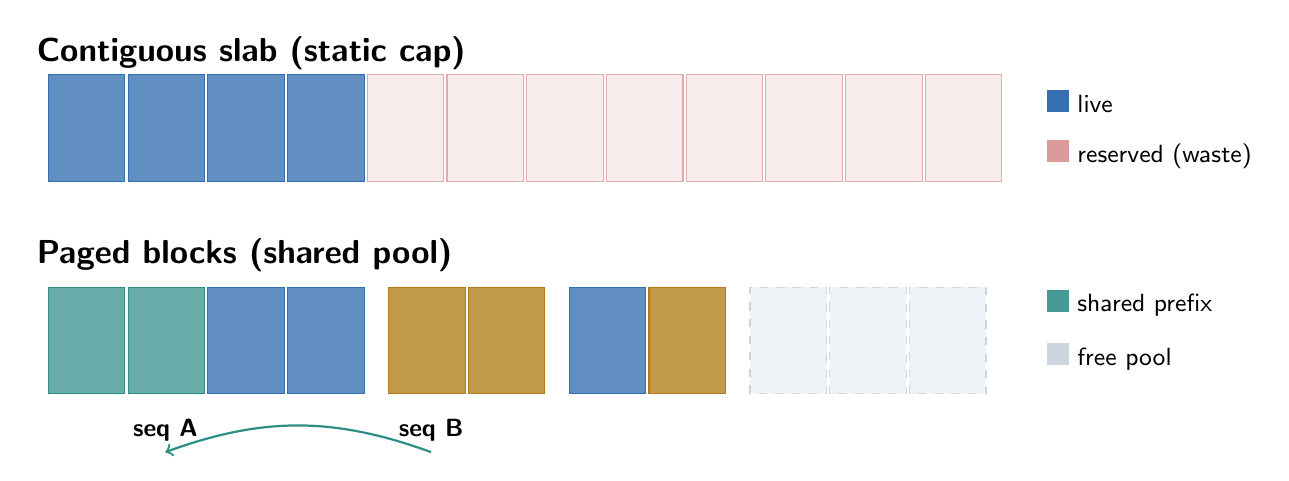
\begin{tikzpicture}[scale=1.35, every node/.style={font=\normalsize}]
      % Contiguous row
      \node[font=\bfseries\large, anchor=west] at (-0.2,2.9) {Contiguous slab (static cap)};
      \foreach \i in {0,...,11} {
            \draw[fill=signalRed!12, draw=signalRed!50] (\i*0.75,1.7) rectangle ++(0.72,1.0);
      }
      \foreach \i in {0,...,3} {
            \draw[fill=signalBlue!70, draw=signalBlue!90] (\i*0.75,1.7) rectangle ++(0.72,1.0);
      }
      \node[anchor=west, font=\small] at (9.3,2.45) {\textcolor{signalBlue!90}{\rule{8pt}{8pt}}\ live};
      \node[anchor=west, font=\small] at (9.3,1.95) {\textcolor{signalRed!60}{\rule{8pt}{8pt}}\ reserved (waste)};

      % Paged row
      \node[font=\bfseries\large, anchor=west] at (-0.2,1.0) {Paged blocks (shared pool)};
      \draw[fill=signalTeal!65, draw=signalTeal!90] (0,-0.3) rectangle ++(0.72,1.0);
      \draw[fill=signalTeal!65, draw=signalTeal!90] (0.75,-0.3) rectangle ++(0.72,1.0);
      \draw[fill=signalBlue!70, draw=signalBlue!90] (1.5,-0.3) rectangle ++(0.72,1.0);
      \draw[fill=signalBlue!70, draw=signalBlue!90] (2.25,-0.3) rectangle ++(0.72,1.0);
      \draw[fill=signalGold!70, draw=signalGold!90] (3.2,-0.3) rectangle ++(0.72,1.0);
      \draw[fill=signalGold!70, draw=signalGold!90] (3.95,-0.3) rectangle ++(0.72,1.0);
      \draw[fill=signalBlue!70, draw=signalBlue!90] (4.9,-0.3) rectangle ++(0.72,1.0);
      \draw[fill=signalGold!70, draw=signalGold!90] (5.65,-0.3) rectangle ++(0.72,1.0);
      \foreach \i in {6.6,7.35,8.1} {
            \draw[fill=panelBg, draw=softBorder, dashed] (\i,-0.3) rectangle ++(0.72,1.0);
      }
      \node[anchor=west, font=\small] at (9.3,0.55) {\textcolor{signalTeal!80}{\rule{8pt}{8pt}}\ shared prefix};
      \node[anchor=west, font=\small] at (9.3,0.05) {\textcolor{softBorder}{\rule{8pt}{8pt}}\ free pool};
      \node[font=\small, anchor=north] at (1.1,-0.45) {\textbf{seq A}};
      \node[font=\small, anchor=north] at (3.6,-0.45) {\textbf{seq B}};
      \draw[->, thick, signalTeal!90] (3.6,-0.85) to[bend right=20] (1.1,-0.85);
\end{tikzpicture}
\end{center}

\subhead{Inference flow}
\begin{enumerate}
      \item \textbf{Prefill:} \texttt{BlockTable} maps logical tokens to physical blocks; K/V written into the pool.
      \item \textbf{Prefix lookup:} hash chain finds the longest reusable prefix; only the suffix runs.
      \item \textbf{Decode / branch:} append to the tail, or fork and pay copy-on-write only on divergence.
      \item \textbf{Retire:} blocks return to the pool when ref counts hit zero.
\end{enumerate}
\end{posterbox}

\blockgap

\begin{posterbox}{signalGold}{\faMemory\ Result 2: Capacity Under Fixed Budget}
\figpanel{figure2.png}
\figcaptiontext{Under the same KV budget, paged allocation fits up to \textbf{2.00x} more concurrent sequences (short prompts) and still \textbf{1.14x} more at 256 tokens.}
\end{posterbox}

\blockgap

\begin{posterbox}{signalGold}{\faHistory\ Result 3: Prefix-Cache Prefill}
\figpanel{figure4.png}
\figcaptiontext{Shared-prefix fractions \textbf{0/25/50/75\%} yield \textbf{1.36x / 1.80x / 1.76x / 1.90x} prefill speedup. Suffixes rotate across trials so gains track real cache hits.}
\end{posterbox}

\blockgap

\begin{posterbox}{signalSlate}{\faInfoCircle\ Measurement Notes}
\bodycopy
\begin{itemize}
      \item Figs.\ 1, 2, 5, 6 are allocator-backed measurements; Fig.\ 4 is timed (1 warmup + 3 trials).
      \item Model: \texttt{n\_embd=512}, \texttt{n\_head=8}, \texttt{n\_layers=4}, \texttt{block\_size=16}, \texttt{num\_kv\_blocks=512}.
      \item Workload mix \texttt{[48,67,112,160,256,80,35,200]}; capacity sweep \texttt{32..256}; prefix sweep \texttt{0/.25/.5/.75}; branching prompts \texttt{32/67/128}.
      \item Synthetic micro-benchmarks isolate allocator behavior; end-to-end latency is future work.
\end{itemize}
\end{posterbox}

\blockgap

\begin{posterbox}{signalSlate}{\faCheckCircle\ Validation}
\bodycopy
\begin{itemize}
      \item \textbf{33 passing tests}; CUDA kernel agrees with the Python reference within \textbf{1e-5}.
      \item Prefill/decode parity verified against shared Q/K/V weights.
\end{itemize}
\end{posterbox}
\end{postercolumn}\hfill
\begin{postercolumn}
\begin{posterbox}{signalTeal}{\faKey\ Key Takeaways}
\bodycopy
One allocator mechanism improves multiple serving bottlenecks at once:
\begin{itemize}
      \item \textbf{Memory:} \textbf{96.6\%} KV efficiency on a realistic mix.
      \item \textbf{Capacity:} up to \textbf{2.00x} more concurrent sequences.
      \item \textbf{Prefix reuse:} up to \textbf{1.90x} faster prefill at 75\% shared.
      \item \textbf{Branch sharing:} \textbf{58--79\%} KV cut for sampling and beams.
      \item \textbf{Implementation setting:} these gains come from a MiniTorch + CUDA prototype, not a paper-only model.
\end{itemize}
\end{posterbox}

\blockgap

\begin{posterbox}{signalGold}{\faChartLine\ Result 4: Parallel-Sampling Memory}
\figpanel{figure5.png}
\figcaptiontext{Forks share the prompt trunk and allocate only divergent decode blocks: \textbf{33--78\%} KV savings, biggest with many outputs from a long shared prompt.}
\end{posterbox}

\blockgap

\begin{posterbox}{signalGold}{\faCubes\ Result 5: Beam-Search Memory}
\figpanel{figure6.png}
\figcaptiontext{Beams share prompt and surviving trunk: peak KV savings \textbf{79\%} at beam width 8, with even less memory after pruning.}
\end{posterbox}

\blockgap

\begin{posterbox}{signalRed}{\faServer\ Serving Implications}
\bodycopy
\begin{itemize}
      \item Better KV efficiency directly increases admission headroom under a fixed memory budget.
      \item Prefix and trunk sharing matter most for multi-output workloads, where many continuations reuse the same prompt.
      \item End-to-end gains still depend on batching, scheduling, and kernel quality, but allocator policy sets the memory ceiling first.
\end{itemize}
\end{posterbox}

\blockgap

\begin{posterbox}{navyDeep}{\faFlag\ Final Takeaway}
{\fontsize{30}{36}\selectfont
Block-granular KV turns worst-case reservation into \textbf{on-demand allocation and sharing} --- delivering more capacity, faster cached prefill, and dramatically cheaper branching from one mechanism. The systems lesson is that better KV residency policy improves throughput, reuse, and branching efficiency without changing the model itself.\par}
\end{posterbox}

\blockgap

\begin{posterbox}{signalSlate}{\faHandshake\ Acknowledgments}
\bodycopy
We thank the \textbf{11-868 LLM Systems} course staff at Carnegie Mellon University for guidance, and the \textbf{MiniTorch} project and the original \textbf{vLLM / PagedAttention} work (Kwon et al., SOSP 2023) for the framework and design we built upon.
\end{posterbox}
\end{postercolumn}

\vspace{0.4mm}

% =====================================================================
% Footer
% =====================================================================
\begin{tcolorbox}[enhanced, arc=4mm,
      colback=navyDeep, colframe=navyDeep, boxrule=0pt,
      left=14mm, right=14mm, top=2.6mm, bottom=2.6mm,
      before skip=0pt, after skip=0pt]
\color{white}\normalsize
\begin{minipage}[t]{0.30\linewidth}
\textbf{\faGithub\ Code} \texttt{11868-course-project}
\end{minipage}\hfill
\begin{minipage}[t]{0.42\linewidth}\centering
\textbf{Keywords} \; PagedAttention \;\(\cdot\)\; KV Cache \;\(\cdot\)\; Prefix Cache \;\(\cdot\)\; Beam Search \;\(\cdot\)\; MiniTorch
\end{minipage}\hfill
\begin{minipage}[t]{0.24\linewidth}\raggedleft
\textbf{Reference} \; Kwon et al., SOSP 2023
\end{minipage}
\end{tcolorbox}

\end{document}
